% Graphic for TeX using PGF
% Title: /home/luiz/study-selection-phases.dia
% Creator: Dia v0.97.3
% CreationDate: Thu May 24 22:14:20 2018
% For: luiz
% \usepackage{tikz}
% The following commands are not supported in PSTricks at present
% We define them conditionally, so when they are implemented,
% this pgf file will use them.
\ifx\du\undefined
  \newlength{\du}
\fi
\setlength{\du}{15\unitlength}
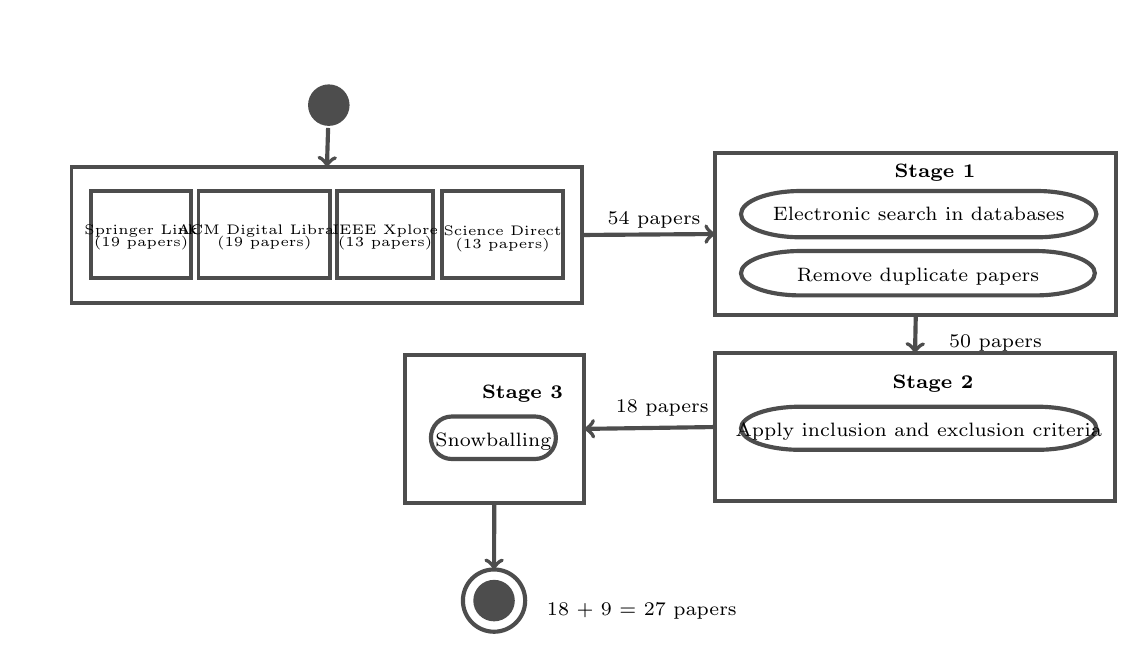
\begin{tikzpicture}
\pgftransformxscale{1.000000}
\pgftransformyscale{-1.000000}
\definecolor{dialinecolor}{rgb}{0.000000, 0.000000, 0.000000}
\pgfsetstrokecolor{dialinecolor}
\definecolor{dialinecolor}{rgb}{1.000000, 1.000000, 1.000000}
\pgfsetfillcolor{dialinecolor}
\definecolor{dialinecolor}{rgb}{1.000000, 1.000000, 1.000000}
\pgfsetfillcolor{dialinecolor}
\fill (-31.917258\du,3.529206\du)--(-31.917258\du,6.807243\du)--(-19.614266\du,6.807243\du)--(-19.614266\du,3.529206\du)--cycle;
\pgfsetlinewidth{0.090000\du}
\pgfsetdash{}{0pt}
\pgfsetdash{}{0pt}
\pgfsetmiterjoin
\definecolor{dialinecolor}{rgb}{0.301961, 0.301961, 0.301961}
\pgfsetstrokecolor{dialinecolor}
\draw (-31.917258\du,3.529206\du)--(-31.917258\du,6.807243\du)--(-19.614266\du,6.807243\du)--(-19.614266\du,3.529206\du)--cycle;
% setfont left to latex
\definecolor{dialinecolor}{rgb}{0.000000, 0.000000, 0.000000}
\pgfsetstrokecolor{dialinecolor}
\node at (-25.765762\du,5.249336\du){};
\definecolor{dialinecolor}{rgb}{1.000000, 1.000000, 1.000000}
\pgfsetfillcolor{dialinecolor}
\fill (-31.448657\du,4.108500\du)--(-31.448657\du,6.196277\du)--(-29.033657\du,6.196277\du)--(-29.033657\du,4.108500\du)--cycle;
\pgfsetlinewidth{0.090000\du}
\pgfsetdash{}{0pt}
\pgfsetdash{}{0pt}
\pgfsetmiterjoin
\definecolor{dialinecolor}{rgb}{0.301961, 0.301961, 0.301961}
\pgfsetstrokecolor{dialinecolor}
\draw (-31.448657\du,4.108500\du)--(-31.448657\du,6.196277\du)--(-29.033657\du,6.196277\du)--(-29.033657\du,4.108500\du)--cycle;
% setfont left to latex
\definecolor{dialinecolor}{rgb}{0.000000, 0.000000, 0.000000}
\pgfsetstrokecolor{dialinecolor}
\node at (-30.241157\du,5.075166\du){\tiny Springer Link};
% setfont left to latex
\definecolor{dialinecolor}{rgb}{0.000000, 0.000000, 0.000000}
\pgfsetstrokecolor{dialinecolor}
\node at (-30.241157\du,5.357389\du){\tiny (19 papers)};
\definecolor{dialinecolor}{rgb}{1.000000, 1.000000, 1.000000}
\pgfsetfillcolor{dialinecolor}
\fill (-28.859928\du,4.108500\du)--(-28.859928\du,6.196277\du)--(-25.689668\du,6.196277\du)--(-25.689668\du,4.108500\du)--cycle;
\pgfsetlinewidth{0.090000\du}
\pgfsetdash{}{0pt}
\pgfsetdash{}{0pt}
\pgfsetmiterjoin
\definecolor{dialinecolor}{rgb}{0.301961, 0.301961, 0.301961}
\pgfsetstrokecolor{dialinecolor}
\draw (-28.859928\du,4.108500\du)--(-28.859928\du,6.196277\du)--(-25.689668\du,6.196277\du)--(-25.689668\du,4.108500\du)--cycle;
% setfont left to latex
\definecolor{dialinecolor}{rgb}{0.000000, 0.000000, 0.000000}
\pgfsetstrokecolor{dialinecolor}
\node at (-27.274798\du,5.075166\du){\tiny ACM Digital Library};
% setfont left to latex
\definecolor{dialinecolor}{rgb}{0.000000, 0.000000, 0.000000}
\pgfsetstrokecolor{dialinecolor}
\node at (-27.274798\du,5.357389\du){\tiny (19 papers)};
% setfont left to latex
\definecolor{dialinecolor}{rgb}{0.000000, 0.000000, 0.000000}
\pgfsetstrokecolor{dialinecolor}
\node[anchor=west] at (-27.274798\du,5.152389\du){};
\definecolor{dialinecolor}{rgb}{1.000000, 1.000000, 1.000000}
\pgfsetfillcolor{dialinecolor}
\fill (-25.520498\du,4.108500\du)--(-25.520498\du,6.196277\du)--(-23.205498\du,6.196277\du)--(-23.205498\du,4.108500\du)--cycle;
\pgfsetlinewidth{0.090000\du}
\pgfsetdash{}{0pt}
\pgfsetdash{}{0pt}
\pgfsetmiterjoin
\definecolor{dialinecolor}{rgb}{0.301961, 0.301961, 0.301961}
\pgfsetstrokecolor{dialinecolor}
\draw (-25.520498\du,4.108500\du)--(-25.520498\du,6.196277\du)--(-23.205498\du,6.196277\du)--(-23.205498\du,4.108500\du)--cycle;
% setfont left to latex
\definecolor{dialinecolor}{rgb}{0.000000, 0.000000, 0.000000}
\pgfsetstrokecolor{dialinecolor}
\node at (-24.362998\du,5.075166\du){\tiny IEEE Xplore};
% setfont left to latex
\definecolor{dialinecolor}{rgb}{0.000000, 0.000000, 0.000000}
\pgfsetstrokecolor{dialinecolor}
\node at (-24.362998\du,5.357389\du){\tiny (13 papers)};
\definecolor{dialinecolor}{rgb}{1.000000, 1.000000, 1.000000}
\pgfsetfillcolor{dialinecolor}
\fill (-22.986880\du,4.108500\du)--(-22.986880\du,6.196277\du)--(-20.079380\du,6.196277\du)--(-20.079380\du,4.108500\du)--cycle;
\pgfsetlinewidth{0.090000\du}
\pgfsetdash{}{0pt}
\pgfsetdash{}{0pt}
\pgfsetmiterjoin
\definecolor{dialinecolor}{rgb}{0.301961, 0.301961, 0.301961}
\pgfsetstrokecolor{dialinecolor}
\draw (-22.986880\du,4.108500\du)--(-22.986880\du,6.196277\du)--(-20.079380\du,6.196277\du)--(-20.079380\du,4.108500\du)--cycle;
% setfont left to latex
\definecolor{dialinecolor}{rgb}{0.000000, 0.000000, 0.000000}
\pgfsetstrokecolor{dialinecolor}
\node at (-21.533130\du,5.057111\du){\tiny Science Direct};
% setfont left to latex
\definecolor{dialinecolor}{rgb}{0.000000, 0.000000, 0.000000}
\pgfsetstrokecolor{dialinecolor}
\node at (-21.533130\du,5.409889\du){\tiny (13 papers)};
\definecolor{dialinecolor}{rgb}{1.000000, 1.000000, 1.000000}
\pgfsetfillcolor{dialinecolor}
\fill (-16.409595\du,3.197689\du)--(-16.409595\du,7.093022\du)--(-6.750481\du,7.093022\du)--(-6.750481\du,3.197689\du)--cycle;
\pgfsetlinewidth{0.090000\du}
\pgfsetdash{}{0pt}
\pgfsetdash{}{0pt}
\pgfsetmiterjoin
\definecolor{dialinecolor}{rgb}{0.301961, 0.301961, 0.301961}
\pgfsetstrokecolor{dialinecolor}
\draw (-16.409595\du,3.197689\du)--(-16.409595\du,7.093022\du)--(-6.750481\du,7.093022\du)--(-6.750481\du,3.197689\du)--cycle;
% setfont left to latex
\definecolor{dialinecolor}{rgb}{0.000000, 0.000000, 0.000000}
\pgfsetstrokecolor{dialinecolor}
\node at (-11.580038\du,4.168133\du){};
% setfont left to latex
\definecolor{dialinecolor}{rgb}{0.000000, 0.000000, 0.000000}
\pgfsetstrokecolor{dialinecolor}
\node at (-11.580038\du,4.520911\du){};
% setfont left to latex
\definecolor{dialinecolor}{rgb}{0.000000, 0.000000, 0.000000}
\pgfsetstrokecolor{dialinecolor}
\node at (-11.580038\du,4.873689\du){};
% setfont left to latex
\definecolor{dialinecolor}{rgb}{0.000000, 0.000000, 0.000000}
\pgfsetstrokecolor{dialinecolor}
\node at (-11.580038\du,5.226466\du){};
% setfont left to latex
\definecolor{dialinecolor}{rgb}{0.000000, 0.000000, 0.000000}
\pgfsetstrokecolor{dialinecolor}
\node at (-11.580038\du,5.579244\du){};
% setfont left to latex
\definecolor{dialinecolor}{rgb}{0.000000, 0.000000, 0.000000}
\pgfsetstrokecolor{dialinecolor}
\node at (-11.580038\du,5.932022\du){};
% setfont left to latex
\definecolor{dialinecolor}{rgb}{0.000000, 0.000000, 0.000000}
\pgfsetstrokecolor{dialinecolor}
\node at (-11.580038\du,6.284800\du){};
% setfont left to latex
\definecolor{dialinecolor}{rgb}{0.000000, 0.000000, 0.000000}
\pgfsetstrokecolor{dialinecolor}
\node[anchor=west] at (-14.727183\du,10.833293\du){};
% setfont left to latex
\definecolor{dialinecolor}{rgb}{0.000000, 0.000000, 0.000000}
\pgfsetstrokecolor{dialinecolor}
\node[anchor=west] at (-11.580038\du,5.145355\du){};
\definecolor{dialinecolor}{rgb}{1.000000, 1.000000, 1.000000}
\pgfsetfillcolor{dialinecolor}
\fill (-16.409595\du,8.014929\du)--(-16.409595\du,11.574374\du)--(-6.787316\du,11.574374\du)--(-6.787316\du,8.014929\du)--cycle;
\pgfsetlinewidth{0.090000\du}
\pgfsetdash{}{0pt}
\pgfsetdash{}{0pt}
\pgfsetmiterjoin
\definecolor{dialinecolor}{rgb}{0.301961, 0.301961, 0.301961}
\pgfsetstrokecolor{dialinecolor}
\draw (-16.409595\du,8.014929\du)--(-16.409595\du,11.574374\du)--(-6.787316\du,11.574374\du)--(-6.787316\du,8.014929\du)--cycle;
% setfont left to latex
\definecolor{dialinecolor}{rgb}{0.000000, 0.000000, 0.000000}
\pgfsetstrokecolor{dialinecolor}
\node at (-11.598455\du,8.817429\du){};
% setfont left to latex
\definecolor{dialinecolor}{rgb}{0.000000, 0.000000, 0.000000}
\pgfsetstrokecolor{dialinecolor}
\node at (-11.598455\du,9.170207\du){};
% setfont left to latex
\definecolor{dialinecolor}{rgb}{0.000000, 0.000000, 0.000000}
\pgfsetstrokecolor{dialinecolor}
\node at (-11.598455\du,9.522985\du){};
% setfont left to latex
\definecolor{dialinecolor}{rgb}{0.000000, 0.000000, 0.000000}
\pgfsetstrokecolor{dialinecolor}
\node at (-11.598455\du,9.875763\du){};
% setfont left to latex
\definecolor{dialinecolor}{rgb}{0.000000, 0.000000, 0.000000}
\pgfsetstrokecolor{dialinecolor}
\node at (-11.598455\du,10.228540\du){};
% setfont left to latex
\definecolor{dialinecolor}{rgb}{0.000000, 0.000000, 0.000000}
\pgfsetstrokecolor{dialinecolor}
\node at (-11.598455\du,10.581318\du){};
% setfont left to latex
\definecolor{dialinecolor}{rgb}{0.000000, 0.000000, 0.000000}
\pgfsetstrokecolor{dialinecolor}
\node at (-11.598455\du,10.934096\du){};
% setfont left to latex
\definecolor{dialinecolor}{rgb}{0.000000, 0.000000, 0.000000}
\pgfsetstrokecolor{dialinecolor}
\node[anchor=west] at (-11.598455\du,9.794652\du){};
% setfont left to latex
\definecolor{dialinecolor}{rgb}{0.000000, 0.000000, 0.000000}
\pgfsetstrokecolor{dialinecolor}
\node[anchor=west] at (-12.122732\du,8.459829\du){};
% setfont left to latex
\definecolor{dialinecolor}{rgb}{0.000000, 0.000000, 0.000000}
\pgfsetstrokecolor{dialinecolor}
\node[anchor=west] at (-15.897732\du,9.584829\du){};
% setfont left to latex
\definecolor{dialinecolor}{rgb}{0.000000, 0.000000, 0.000000}
\pgfsetstrokecolor{dialinecolor}
\node[anchor=west] at (-12.154697\du,8.372549\du){};
% setfont left to latex
\definecolor{dialinecolor}{rgb}{0.000000, 0.000000, 0.000000}
\pgfsetstrokecolor{dialinecolor}
\node[anchor=west] at (-11.598455\du,9.794652\du){};
% setfont left to latex
\definecolor{dialinecolor}{rgb}{0.000000, 0.000000, 0.000000}
\pgfsetstrokecolor{dialinecolor}
\node[anchor=west] at (-12.974637\du,7.860073\du){};
% setfont left to latex
\definecolor{dialinecolor}{rgb}{0.000000, 0.000000, 0.000000}
\pgfsetstrokecolor{dialinecolor}
\node[anchor=west] at (-14.979697\du,8.522549\du){};
% setfont left to latex
\definecolor{dialinecolor}{rgb}{0.000000, 0.000000, 0.000000}
\pgfsetstrokecolor{dialinecolor}
\node[anchor=west] at (-10.466532\du,8.591129\du){};
\definecolor{dialinecolor}{rgb}{1.000000, 1.000000, 1.000000}
\pgfsetfillcolor{dialinecolor}
\fill (-23.887162\du,8.059949\du)--(-23.887162\du,11.619393\du)--(-19.569166\du,11.619393\du)--(-19.569166\du,8.059949\du)--cycle;
\pgfsetlinewidth{0.090000\du}
\pgfsetdash{}{0pt}
\pgfsetdash{}{0pt}
\pgfsetmiterjoin
\definecolor{dialinecolor}{rgb}{0.301961, 0.301961, 0.301961}
\pgfsetstrokecolor{dialinecolor}
\draw (-23.887162\du,8.059949\du)--(-23.887162\du,11.619393\du)--(-19.569166\du,11.619393\du)--(-19.569166\du,8.059949\du)--cycle;
% setfont left to latex
\definecolor{dialinecolor}{rgb}{0.000000, 0.000000, 0.000000}
\pgfsetstrokecolor{dialinecolor}
\node at (-21.728164\du,8.862449\du){};
% setfont left to latex
\definecolor{dialinecolor}{rgb}{0.000000, 0.000000, 0.000000}
\pgfsetstrokecolor{dialinecolor}
\node at (-21.728164\du,9.215226\du){};
% setfont left to latex
\definecolor{dialinecolor}{rgb}{0.000000, 0.000000, 0.000000}
\pgfsetstrokecolor{dialinecolor}
\node at (-21.728164\du,9.568004\du){};
% setfont left to latex
\definecolor{dialinecolor}{rgb}{0.000000, 0.000000, 0.000000}
\pgfsetstrokecolor{dialinecolor}
\node at (-21.728164\du,9.920782\du){};
% setfont left to latex
\definecolor{dialinecolor}{rgb}{0.000000, 0.000000, 0.000000}
\pgfsetstrokecolor{dialinecolor}
\node at (-21.728164\du,10.273560\du){};
% setfont left to latex
\definecolor{dialinecolor}{rgb}{0.000000, 0.000000, 0.000000}
\pgfsetstrokecolor{dialinecolor}
\node at (-21.728164\du,10.626338\du){};
% setfont left to latex
\definecolor{dialinecolor}{rgb}{0.000000, 0.000000, 0.000000}
\pgfsetstrokecolor{dialinecolor}
\node at (-21.728164\du,10.979115\du){};
% setfont left to latex
\definecolor{dialinecolor}{rgb}{0.000000, 0.000000, 0.000000}
\pgfsetstrokecolor{dialinecolor}
\node[anchor=west] at (-21.728164\du,9.839671\du){};
% setfont left to latex
\definecolor{dialinecolor}{rgb}{0.000000, 0.000000, 0.000000}
\pgfsetstrokecolor{dialinecolor}
\node[anchor=west] at (-22.296676\du,9.004456\du){\scriptsize \textbf{Stage 3}};
% setfont left to latex
\definecolor{dialinecolor}{rgb}{0.000000, 0.000000, 0.000000}
\pgfsetstrokecolor{dialinecolor}
\node[anchor=west] at (-17.469006\du,11.002467\du){};
% setfont left to latex
\definecolor{dialinecolor}{rgb}{0.000000, 0.000000, 0.000000}
\pgfsetstrokecolor{dialinecolor}
\node[anchor=west] at (-22.385901\du,10.417810\du){};
% setfont left to latex
\definecolor{dialinecolor}{rgb}{0.000000, 0.000000, 0.000000}
\pgfsetstrokecolor{dialinecolor}
\node[anchor=west] at (-21.728164\du,9.839671\du){};
% setfont left to latex
\definecolor{dialinecolor}{rgb}{0.000000, 0.000000, 0.000000}
\pgfsetstrokecolor{dialinecolor}
\node[anchor=west] at (-30.104804\du,11.393752\du){};
% setfont left to latex
\definecolor{dialinecolor}{rgb}{0.000000, 0.000000, 0.000000}
\pgfsetstrokecolor{dialinecolor}
\node[anchor=west] at (-26.271407\du,8.805627\du){};
% setfont left to latex
\definecolor{dialinecolor}{rgb}{0.000000, 0.000000, 0.000000}
\pgfsetstrokecolor{dialinecolor}
\node[anchor=west] at (-21.985901\du,10.425310\du){};
\pgfsetlinewidth{0.100000\du}
\pgfsetdash{}{0pt}
\pgfsetdash{}{0pt}
\pgfsetbuttcap
\pgfsetmiterjoin
\pgfsetlinewidth{0.100000\du}
\pgfsetbuttcap
\pgfsetmiterjoin
\pgfsetdash{}{0pt}
\definecolor{dialinecolor}{rgb}{1.000000, 1.000000, 1.000000}
\pgfsetfillcolor{dialinecolor}
\pgfpathmoveto{\pgfpoint{-14.364235\du}{4.109362\du}}
\pgfpathlineto{\pgfpoint{-8.656319\du}{4.109362\du}}
\pgfpathcurveto{\pgfpoint{-7.868219\du}{4.109362\du}}{\pgfpoint{-7.229340\du}{4.358800\du}}{\pgfpoint{-7.229340\du}{4.666496\du}}
\pgfpathcurveto{\pgfpoint{-7.229340\du}{4.974193\du}}{\pgfpoint{-7.868219\du}{5.223630\du}}{\pgfpoint{-8.656319\du}{5.223630\du}}
\pgfpathlineto{\pgfpoint{-14.364235\du}{5.223630\du}}
\pgfpathcurveto{\pgfpoint{-15.152334\du}{5.223630\du}}{\pgfpoint{-15.791214\du}{4.974193\du}}{\pgfpoint{-15.791214\du}{4.666496\du}}
\pgfpathcurveto{\pgfpoint{-15.791214\du}{4.358800\du}}{\pgfpoint{-15.152334\du}{4.109362\du}}{\pgfpoint{-14.364235\du}{4.109362\du}}
\pgfusepath{fill}
\definecolor{dialinecolor}{rgb}{0.301961, 0.301961, 0.301961}
\pgfsetstrokecolor{dialinecolor}
\pgfpathmoveto{\pgfpoint{-14.364235\du}{4.109362\du}}
\pgfpathlineto{\pgfpoint{-8.656319\du}{4.109362\du}}
\pgfpathcurveto{\pgfpoint{-7.868219\du}{4.109362\du}}{\pgfpoint{-7.229340\du}{4.358800\du}}{\pgfpoint{-7.229340\du}{4.666496\du}}
\pgfpathcurveto{\pgfpoint{-7.229340\du}{4.974193\du}}{\pgfpoint{-7.868219\du}{5.223630\du}}{\pgfpoint{-8.656319\du}{5.223630\du}}
\pgfpathlineto{\pgfpoint{-14.364235\du}{5.223630\du}}
\pgfpathcurveto{\pgfpoint{-15.152334\du}{5.223630\du}}{\pgfpoint{-15.791214\du}{4.974193\du}}{\pgfpoint{-15.791214\du}{4.666496\du}}
\pgfpathcurveto{\pgfpoint{-15.791214\du}{4.358800\du}}{\pgfpoint{-15.152334\du}{4.109362\du}}{\pgfpoint{-14.364235\du}{4.109362\du}}
\pgfusepath{stroke}
% setfont left to latex
\definecolor{dialinecolor}{rgb}{0.000000, 0.000000, 0.000000}
\pgfsetstrokecolor{dialinecolor}
\node at (-11.510277\du,4.654691\du){\scriptsize Electronic search in databases};
% setfont left to latex
\definecolor{dialinecolor}{rgb}{0.000000, 0.000000, 0.000000}
\pgfsetstrokecolor{dialinecolor}
\node[anchor=west] at (-11.510277\du,4.666496\du){};
% setfont left to latex
\definecolor{dialinecolor}{rgb}{0.000000, 0.000000, 0.000000}
\pgfsetstrokecolor{dialinecolor}
\node[anchor=west] at (-11.580038\du,5.145355\du){};
\pgfsetlinewidth{0.100000\du}
\pgfsetdash{}{0pt}
\pgfsetdash{}{0pt}
\pgfsetbuttcap
\pgfsetmiterjoin
\pgfsetlinewidth{0.100000\du}
\pgfsetbuttcap
\pgfsetmiterjoin
\pgfsetdash{}{0pt}
\definecolor{dialinecolor}{rgb}{1.000000, 1.000000, 1.000000}
\pgfsetfillcolor{dialinecolor}
\pgfpathmoveto{\pgfpoint{-14.370374\du}{5.555148\du}}
\pgfpathlineto{\pgfpoint{-8.687015\du}{5.555148\du}}
\pgfpathcurveto{\pgfpoint{-7.902306\du}{5.555148\du}}{\pgfpoint{-7.266175\du}{5.794278\du}}{\pgfpoint{-7.266175\du}{6.089260\du}}
\pgfpathcurveto{\pgfpoint{-7.266175\du}{6.384242\du}}{\pgfpoint{-7.902306\du}{6.623372\du}}{\pgfpoint{-8.687015\du}{6.623372\du}}
\pgfpathlineto{\pgfpoint{-14.370374\du}{6.623372\du}}
\pgfpathcurveto{\pgfpoint{-15.155083\du}{6.623372\du}}{\pgfpoint{-15.791214\du}{6.384242\du}}{\pgfpoint{-15.791214\du}{6.089260\du}}
\pgfpathcurveto{\pgfpoint{-15.791214\du}{5.794278\du}}{\pgfpoint{-15.155083\du}{5.555148\du}}{\pgfpoint{-14.370374\du}{5.555148\du}}
\pgfusepath{fill}
\definecolor{dialinecolor}{rgb}{0.301961, 0.301961, 0.301961}
\pgfsetstrokecolor{dialinecolor}
\pgfpathmoveto{\pgfpoint{-14.370374\du}{5.555148\du}}
\pgfpathlineto{\pgfpoint{-8.687015\du}{5.555148\du}}
\pgfpathcurveto{\pgfpoint{-7.902306\du}{5.555148\du}}{\pgfpoint{-7.266175\du}{5.794278\du}}{\pgfpoint{-7.266175\du}{6.089260\du}}
\pgfpathcurveto{\pgfpoint{-7.266175\du}{6.384242\du}}{\pgfpoint{-7.902306\du}{6.623372\du}}{\pgfpoint{-8.687015\du}{6.623372\du}}
\pgfpathlineto{\pgfpoint{-14.370374\du}{6.623372\du}}
\pgfpathcurveto{\pgfpoint{-15.155083\du}{6.623372\du}}{\pgfpoint{-15.791214\du}{6.384242\du}}{\pgfpoint{-15.791214\du}{6.089260\du}}
\pgfpathcurveto{\pgfpoint{-15.791214\du}{5.794278\du}}{\pgfpoint{-15.155083\du}{5.555148\du}}{\pgfpoint{-14.370374\du}{5.555148\du}}
\pgfusepath{stroke}
% setfont left to latex
\definecolor{dialinecolor}{rgb}{0.000000, 0.000000, 0.000000}
\pgfsetstrokecolor{dialinecolor}
\node at (-11.528694\du,6.177454\du){\scriptsize Remove duplicate papers};
% setfont left to latex
\definecolor{dialinecolor}{rgb}{0.000000, 0.000000, 0.000000}
\pgfsetstrokecolor{dialinecolor}
\node[anchor=west] at (-11.510277\du,4.666496\du){};
\pgfsetlinewidth{0.100000\du}
\pgfsetdash{}{0pt}
\pgfsetdash{}{0pt}
\pgfsetbuttcap
\pgfsetmiterjoin
\pgfsetlinewidth{0.100000\du}
\pgfsetbuttcap
\pgfsetmiterjoin
\pgfsetdash{}{0pt}
\definecolor{dialinecolor}{rgb}{1.000000, 1.000000, 1.000000}
\pgfsetfillcolor{dialinecolor}
\pgfpathmoveto{\pgfpoint{-14.364235\du}{9.305335\du}}
\pgfpathlineto{\pgfpoint{-8.656319\du}{9.305335\du}}
\pgfpathcurveto{\pgfpoint{-7.868219\du}{9.305335\du}}{\pgfpoint{-7.229340\du}{9.537789\du}}{\pgfpoint{-7.229340\du}{9.824536\du}}
\pgfpathcurveto{\pgfpoint{-7.229340\du}{10.111283\du}}{\pgfpoint{-7.868219\du}{10.343738\du}}{\pgfpoint{-8.656319\du}{10.343738\du}}
\pgfpathlineto{\pgfpoint{-14.364235\du}{10.343738\du}}
\pgfpathcurveto{\pgfpoint{-15.152334\du}{10.343738\du}}{\pgfpoint{-15.791214\du}{10.111283\du}}{\pgfpoint{-15.791214\du}{9.824536\du}}
\pgfpathcurveto{\pgfpoint{-15.791214\du}{9.537789\du}}{\pgfpoint{-15.152334\du}{9.305335\du}}{\pgfpoint{-14.364235\du}{9.305335\du}}
\pgfusepath{fill}
\definecolor{dialinecolor}{rgb}{0.301961, 0.301961, 0.301961}
\pgfsetstrokecolor{dialinecolor}
\pgfpathmoveto{\pgfpoint{-14.364235\du}{9.305335\du}}
\pgfpathlineto{\pgfpoint{-8.656319\du}{9.305335\du}}
\pgfpathcurveto{\pgfpoint{-7.868219\du}{9.305335\du}}{\pgfpoint{-7.229340\du}{9.537789\du}}{\pgfpoint{-7.229340\du}{9.824536\du}}
\pgfpathcurveto{\pgfpoint{-7.229340\du}{10.111283\du}}{\pgfpoint{-7.868219\du}{10.343738\du}}{\pgfpoint{-8.656319\du}{10.343738\du}}
\pgfpathlineto{\pgfpoint{-14.364235\du}{10.343738\du}}
\pgfpathcurveto{\pgfpoint{-15.152334\du}{10.343738\du}}{\pgfpoint{-15.791214\du}{10.111283\du}}{\pgfpoint{-15.791214\du}{9.824536\du}}
\pgfpathcurveto{\pgfpoint{-15.791214\du}{9.537789\du}}{\pgfpoint{-15.152334\du}{9.305335\du}}{\pgfpoint{-14.364235\du}{9.305335\du}}
\pgfusepath{stroke}
% setfont left to latex
\definecolor{dialinecolor}{rgb}{0.000000, 0.000000, 0.000000}
\pgfsetstrokecolor{dialinecolor}
\node at (-11.510277\du,9.912731\du){\scriptsize Apply inclusion and exclusion criteria};
\pgfsetlinewidth{0.100000\du}
\pgfsetdash{}{0pt}
\pgfsetdash{}{0pt}
\pgfsetbuttcap
\pgfsetmiterjoin
\pgfsetlinewidth{0.100000\du}
\pgfsetbuttcap
\pgfsetmiterjoin
\pgfsetdash{}{0pt}
\definecolor{dialinecolor}{rgb}{1.000000, 1.000000, 1.000000}
\pgfsetfillcolor{dialinecolor}
\pgfpathmoveto{\pgfpoint{-22.759086\du}{9.541292\du}}
\pgfpathlineto{\pgfpoint{-20.751586\du}{9.541292\du}}
\pgfpathcurveto{\pgfpoint{-20.474408\du}{9.541292\du}}{\pgfpoint{-20.249711\du}{9.770400\du}}{\pgfpoint{-20.249711\du}{10.053021\du}}
\pgfpathcurveto{\pgfpoint{-20.249711\du}{10.335641\du}}{\pgfpoint{-20.474408\du}{10.564749\du}}{\pgfpoint{-20.751586\du}{10.564749\du}}
\pgfpathlineto{\pgfpoint{-22.759086\du}{10.564749\du}}
\pgfpathcurveto{\pgfpoint{-23.036264\du}{10.564749\du}}{\pgfpoint{-23.260961\du}{10.335641\du}}{\pgfpoint{-23.260961\du}{10.053021\du}}
\pgfpathcurveto{\pgfpoint{-23.260961\du}{9.770400\du}}{\pgfpoint{-23.036264\du}{9.541292\du}}{\pgfpoint{-22.759086\du}{9.541292\du}}
\pgfusepath{fill}
\definecolor{dialinecolor}{rgb}{0.301961, 0.301961, 0.301961}
\pgfsetstrokecolor{dialinecolor}
\pgfpathmoveto{\pgfpoint{-22.759086\du}{9.541292\du}}
\pgfpathlineto{\pgfpoint{-20.751586\du}{9.541292\du}}
\pgfpathcurveto{\pgfpoint{-20.474408\du}{9.541292\du}}{\pgfpoint{-20.249711\du}{9.770400\du}}{\pgfpoint{-20.249711\du}{10.053021\du}}
\pgfpathcurveto{\pgfpoint{-20.249711\du}{10.335641\du}}{\pgfpoint{-20.474408\du}{10.564749\du}}{\pgfpoint{-20.751586\du}{10.564749\du}}
\pgfpathlineto{\pgfpoint{-22.759086\du}{10.564749\du}}
\pgfpathcurveto{\pgfpoint{-23.036264\du}{10.564749\du}}{\pgfpoint{-23.260961\du}{10.335641\du}}{\pgfpoint{-23.260961\du}{10.053021\du}}
\pgfpathcurveto{\pgfpoint{-23.260961\du}{9.770400\du}}{\pgfpoint{-23.036264\du}{9.541292\du}}{\pgfpoint{-22.759086\du}{9.541292\du}}
\pgfusepath{stroke}
% setfont left to latex
\definecolor{dialinecolor}{rgb}{0.000000, 0.000000, 0.000000}
\pgfsetstrokecolor{dialinecolor}
\node at (-21.755336\du,10.141215\du){\scriptsize Snowballing};
\pgfsetlinewidth{0.100000\du}
\pgfsetdash{}{0pt}
\pgfsetdash{}{0pt}
\pgfsetbuttcap
{
\definecolor{dialinecolor}{rgb}{0.301961, 0.301961, 0.301961}
\pgfsetfillcolor{dialinecolor}
% was here!!!
\pgfsetarrowsend{to}
\definecolor{dialinecolor}{rgb}{0.301961, 0.301961, 0.301961}
\pgfsetstrokecolor{dialinecolor}
\draw (-19.614266\du,5.168224\du)--(-16.409595\du,5.145355\du);
}
\pgfsetlinewidth{0.100000\du}
\pgfsetdash{}{0pt}
\pgfsetdash{}{0pt}
\pgfsetbuttcap
{
\definecolor{dialinecolor}{rgb}{0.301961, 0.301961, 0.301961}
\pgfsetfillcolor{dialinecolor}
% was here!!!
\pgfsetarrowsend{to}
\definecolor{dialinecolor}{rgb}{0.301961, 0.301961, 0.301961}
\pgfsetstrokecolor{dialinecolor}
\draw (-11.580038\du,7.093022\du)--(-11.598455\du,8.014929\du);
}
\pgfsetlinewidth{0.100000\du}
\pgfsetdash{}{0pt}
\pgfsetdash{}{0pt}
\pgfsetbuttcap
{
\definecolor{dialinecolor}{rgb}{0.301961, 0.301961, 0.301961}
\pgfsetfillcolor{dialinecolor}
% was here!!!
\pgfsetarrowsend{to}
\definecolor{dialinecolor}{rgb}{0.301961, 0.301961, 0.301961}
\pgfsetstrokecolor{dialinecolor}
\draw (-16.409595\du,9.794652\du)--(-19.569166\du,9.839671\du);
}
% setfont left to latex
\definecolor{dialinecolor}{rgb}{0.301961, 0.301961, 0.301961}
\pgfsetstrokecolor{dialinecolor}
\node[anchor=west] at (-19.275615\du,4.813556\du){\scriptsize 54 papers};
% setfont left to latex
\definecolor{dialinecolor}{rgb}{0.301961, 0.301961, 0.301961}
\pgfsetstrokecolor{dialinecolor}
\node[anchor=west] at (-11.052270\du,7.784965\du){\scriptsize 50 papers};
% setfont left to latex
\definecolor{dialinecolor}{rgb}{0.000000, 0.000000, 0.000000}
\pgfsetstrokecolor{dialinecolor}
\node[anchor=west] at (-21.429176\du,7.178609\du){};
% setfont left to latex
\definecolor{dialinecolor}{rgb}{0.301961, 0.301961, 0.301961}
\pgfsetstrokecolor{dialinecolor}
\node[anchor=west] at (-19.080362\du,9.338528\du){\scriptsize 18 papers};
\pgfsetlinewidth{0.100000\du}
\pgfsetdash{}{0pt}
\definecolor{dialinecolor}{rgb}{1.000000, 1.000000, 1.000000}
\pgfsetfillcolor{dialinecolor}
\pgfpathellipse{\pgfpoint{-21.739730\du}{13.975896\du}}{\pgfpoint{0.750000\du}{0\du}}{\pgfpoint{0\du}{0.750000\du}}
\pgfusepath{fill}
\definecolor{dialinecolor}{rgb}{0.301961, 0.301961, 0.301961}
\pgfsetstrokecolor{dialinecolor}
\pgfpathellipse{\pgfpoint{-21.739730\du}{13.975896\du}}{\pgfpoint{0.750000\du}{0\du}}{\pgfpoint{0\du}{0.750000\du}}
\pgfusepath{stroke}
\definecolor{dialinecolor}{rgb}{0.301961, 0.301961, 0.301961}
\pgfsetfillcolor{dialinecolor}
\pgfpathellipse{\pgfpoint{-21.739730\du}{13.975896\du}}{\pgfpoint{0.500000\du}{0\du}}{\pgfpoint{0\du}{0.500000\du}}
\pgfusepath{fill}
\pgfsetlinewidth{0.100000\du}
\pgfsetdash{}{0pt}
\pgfsetdash{}{0pt}
\pgfsetbuttcap
{
\definecolor{dialinecolor}{rgb}{0.301961, 0.301961, 0.301961}
\pgfsetfillcolor{dialinecolor}
% was here!!!
\pgfsetarrowsend{to}
\definecolor{dialinecolor}{rgb}{0.301961, 0.301961, 0.301961}
\pgfsetstrokecolor{dialinecolor}
\draw (-21.734353\du,11.651831\du)--(-21.739730\du,13.225896\du);
}
\pgfsetlinewidth{0.100000\du}
\pgfsetdash{}{0pt}
\definecolor{dialinecolor}{rgb}{0.301961, 0.301961, 0.301961}
\pgfsetfillcolor{dialinecolor}
\pgfpathellipse{\pgfpoint{-25.720406\du}{2.040372\du}}{\pgfpoint{0.500000\du}{0\du}}{\pgfpoint{0\du}{0.500000\du}}
\pgfusepath{fill}
\pgfsetlinewidth{0.100000\du}
\pgfsetdash{}{0pt}
\pgfsetdash{}{0pt}
\pgfsetbuttcap
{
\definecolor{dialinecolor}{rgb}{0.301961, 0.301961, 0.301961}
\pgfsetfillcolor{dialinecolor}
% was here!!!
\pgfsetarrowsend{to}
\definecolor{dialinecolor}{rgb}{0.301961, 0.301961, 0.301961}
\pgfsetstrokecolor{dialinecolor}
\draw (-25.737160\du,2.590325\du)--(-25.765762\du,3.529206\du);
}
% setfont left to latex
\definecolor{dialinecolor}{rgb}{0.000000, 0.000000, 0.000000}
\pgfsetstrokecolor{dialinecolor}
\node[anchor=west] at (-10.434011\du,3.418700\du){};
% setfont left to latex
\definecolor{dialinecolor}{rgb}{0.301961, 0.301961, 0.301961}
\pgfsetstrokecolor{dialinecolor}
\node[anchor=west] at (-20.736845\du,14.238237\du){\scriptsize 18 + 9 = 27 papers};
% setfont left to latex
\definecolor{dialinecolor}{rgb}{0.301961, 0.301961, 0.301961}
\pgfsetstrokecolor{dialinecolor}
\node[anchor=west] at (-31.713766\du,0.646010\du){};
% setfont left to latex
\definecolor{dialinecolor}{rgb}{0.000000, 0.000000, 0.000000}
\pgfsetstrokecolor{dialinecolor}
\node[anchor=west] at (-12.364726\du,3.677517\du){\scriptsize \textbf{Stage 1}};
% setfont left to latex
\definecolor{dialinecolor}{rgb}{0.000000, 0.000000, 0.000000}
\pgfsetstrokecolor{dialinecolor}
\node[anchor=west] at (-11.723247\du,3.750218\du){};
% setfont left to latex
\definecolor{dialinecolor}{rgb}{0.000000, 0.000000, 0.000000}
\pgfsetstrokecolor{dialinecolor}
\node[anchor=west] at (-33.025103\du,0.396474\du){};
% setfont left to latex
\definecolor{dialinecolor}{rgb}{0.000000, 0.000000, 0.000000}
\pgfsetstrokecolor{dialinecolor}
\node[anchor=west] at (-33.025103\du,0.396474\du){};
% setfont left to latex
\definecolor{dialinecolor}{rgb}{0.000000, 0.000000, 0.000000}
\pgfsetstrokecolor{dialinecolor}
\node[anchor=west] at (-12.413156\du,8.757105\du){\scriptsize \textbf{Stage 2}};
\end{tikzpicture}
